\newcommand{\selunsorted}{{80,70,10,10,50,30,90,40}}
\newcommand{\selitera}{{10,70,80,10,50,30,90,40}}
\newcommand{\seliterb}{{10,10,80,70,50,30,90,40}}
\newcommand{\seliterc}{{10,10,30,70,50,80,90,40}}
\newcommand{\seliterd}{{10,10,30,40,50,80,90,70}}
\newcommand{\selitere}{{10,10,30,40,50,80,90,70}}
\newcommand{\seliterf}{{10,10,30,40,50,70,90,80}}
\newcommand{\seliterg}{{10,10,30,40,50,70,80,90}}
\newcommand{\selsorted}{{10,10,30,40,50,70,80,90}}
\tikzstyle{unsorted} = [draw,fill=red!40,minimum size=3.6em]
\tikzstyle{sorted} = [draw,fill=green!90!black,minimum size=3.6em]
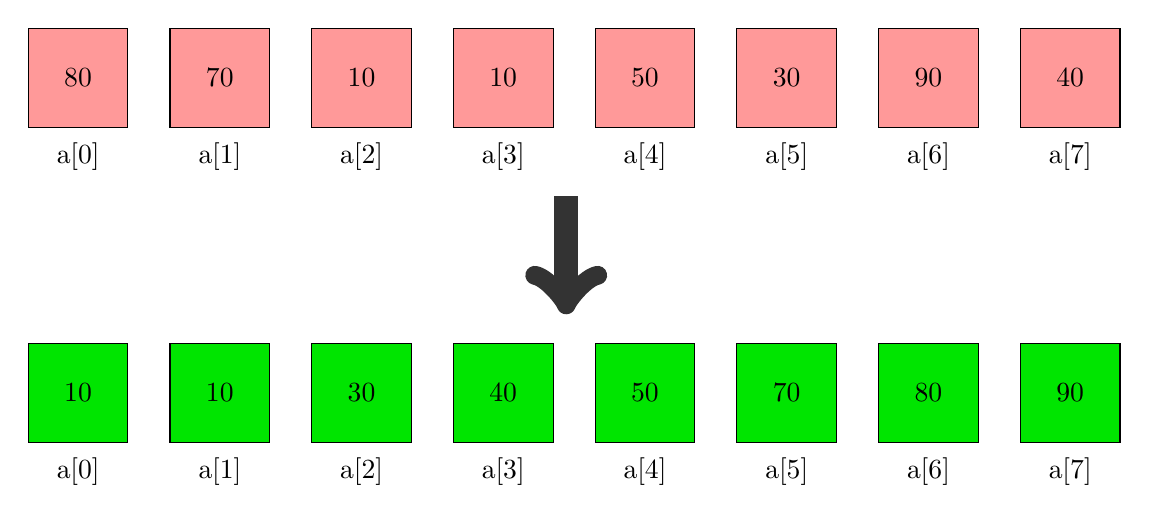
\begin{tikzpicture}
\foreach \x in {0,1,...,7} {
	\node[unsorted] at (\x*1.8,5) (block\x) {\pgfmathparse{\selunsorted[\x]}\pgfmathresult};
	\node at (\x*1.8, 4) {a[\x]};
	
	\node[sorted] at (\x*1.8,1) (block\x) {\pgfmathparse{\selsorted[\x]}\pgfmathresult};
	\node at (\x*1.8, 0) {a[\x]};	
}
	\draw [line width=3mm, ->, black!80!white] (6.2,3.5) -- (6.2, 2);
\end{tikzpicture}